\documentclass[11pt]{utalcaDoc}
\usepackage{alltt}
\usepackage{underscore}
\usepackage[utf8]{inputenc}
\usepackage[activeacute,spanish]{babel}
\usepackage{verbatim}
\usepackage[pdftex]{graphicx}
\usepackage{ae}
\usepackage{amsmath}
\usepackage{amsfonts}
\usepackage{pdflscape}
\usepackage{inconsolata}
\usepackage{url}
\usepackage{hyperref}
\usepackage{listings}
% \usepackage{placeins}
\usepackage[section]{placeins}
\usepackage[stable]{footmisc}


\title{{\bf Seguridad Informática}\\ Tarea 4}

\author{Erik Regla, author 2, author 3\\ 
\{eregla09, author2, author3\}@alumnos.utalca.cl}

\date{\today}
\lstset{language=SH, 
		basicstyle=\ttfamily\tiny, 
		showspaces=false, 
		numbers=left, 
		breaklines=true,
		frame=shadowbox
		}

\begin{document}

\maketitle

\section{Enunciado}
Deberá elegir un tipo de empresa del listado que se presenta. Para
esta empresa ficticia deberá crear una razón social, misión y visión,
organigrama. Además deberá realizar la identificación de los activos
importantes de la empresa (al menos 10 activos).

Deberá entregar un informe con la especificación de los activos que
haya identificado, según lo visto en esta presentación.

Además el Gerente General de la empresa, deberá presentar
los 5 activos más importantes durante la clase, dando énfasis
en la valoración del activo y explicar el porqué de esta
valoración.

\section{Desarrollo}

\subsection{Tipo de empresa elegida}
Consultora - TI\\
ESIL - Empresa de Servicios Informaticos LTDA

\subsection{Misión}
Ser la empresa líder en servicios informaticos de asesoría y desarrollo a nivel nacional para el sector público y privado, entregando de manera contínua una propuesta de valor para su empresa.

\subsection{Visión}
Como empresa líder en el rubro de la consultoría TI nuestros esfuerzos se concentran en estar constantemente actualizados respecto a la vanguardia tecnológica y de seguridad de la información.

En base a esto, nuestro objetivo es contribuir a la construcción de una sociedad más segura y con mayor alcance tecnológico por medio del acercamiento de la misma, de modo que las tecnologías de la información puedan estar disponibles para cualquier organización que lo requiera sin necesidad de mayores complicaciones.

\subsection{Organigrama}
\begin{figure}[ht]
    \centering
    \caption{Organigrama}
    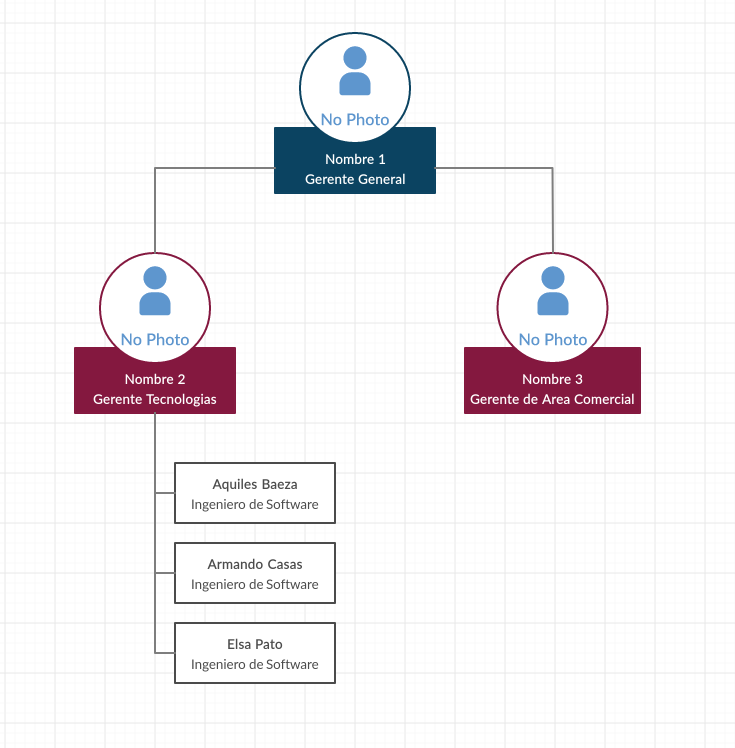
\includegraphics[width=0.5\textwidth]{organigrama.png}
    \label{FIG:ORGANIGRAMA}
\end{figure}

\subsection{Listado de Activos}

\subsubsection{PHY-CEG-001}
\begin{itemize}
    \item {\textbf{Descripción:}   Thinkpad T470s }
    \item {\textbf{Categoría:}     Activo Físico - Hardware TI - Equipo portátil}
    \item {\textbf{Ubicación:}     Oficina }
    \item {\textbf{Propietario:}   Gerente General }
    \item {\textbf{Valoración:}
          \begin{itemize}
              \item Confidencialidad:
              \item Integridad:
              \item Disponibilidad:
              \item Total:
          \end{itemize}
          }
\end{itemize}

\subsubsection{PHY-SRV-01}
\begin{itemize}
    \item {\textbf{Descripción:}   Servidor de desarrollo }
    \item {\textbf{Categoría:}     Activo Físico - Hardware TI - Servidor}
    \item {\textbf{Ubicación:}     Oficina }
    \item {\textbf{Propietario:}   Organización } %consultar quien es dueño de que cosa acá
    \item {\textbf{Valoración:}
          \begin{itemize}
              \item Confidencialidad:
              \item Integridad:
              \item Disponibilidad:
              \item Total:
          \end{itemize}
          }
\end{itemize}

\subsubsection{PHY-BLD-01}
\begin{itemize}
    \item {\textbf{Descripción:}   Oficina 74 }
    \item {\textbf{Categoría:}     Activo Físico - Infraestructura TI - Oficina}
    \item {\textbf{Ubicación:}     Antonio Bellet 10 - Providencia - Santiago }
    \item {\textbf{Propietario:}   Inmobiliaria Ensueño } %consultar quien es dueño de que cosa acá
    \item {\textbf{Valoración:}
          \begin{itemize}
              \item Confidencialidad:
              \item Integridad:
              \item Disponibilidad:
              \item Total:
          \end{itemize}
          }
\end{itemize}


\subsubsection{SW-CLOUD-001}
\begin{itemize}
    \item {\textbf{Descripción:}   Cuenta Google Suite corporativa }
    \item {\textbf{Categoría:}     Activo de Servicios de TI - Nube corporativa}
    \item {\textbf{Ubicación:}     Nube de Google }
    \item {\textbf{Propietario:}   Organización } %consultar quien es dueño de que cosa acá
    \item {\textbf{Valoración:}
          \begin{itemize}
              \item Confidencialidad:
              \item Integridad:
              \item Disponibilidad:
              \item Total:
          \end{itemize}
          }
\end{itemize}

\subsubsection{SW-DB-001}
\begin{itemize}
    \item {\textbf{Descripción:}   Base de datos para desarrollo interno }
    \item {\textbf{Categoría:}     Activo de Información - Base de datos}
    \item {\textbf{Ubicación:}     Oficina - PHY-SRV-01 }
    \item {\textbf{Propietario:}   Organización } %consultar quien es dueño de que cosa acá
    \item {\textbf{Valoración:}
          \begin{itemize}
              \item Confidencialidad:
              \item Integridad:
              \item Disponibilidad:
              \item Total:
          \end{itemize}
          }
\end{itemize}

\subsubsection{PT-CPRH-001}
\begin{itemize}
    \item {\textbf{Descripción:}   Patente prototipo firewall para dispositivos Xtensa }
    \item {\textbf{Categoría:}     Activo de Información - Intangible - patente}
    \item {\textbf{Ubicación:}     INAPI }
    \item {\textbf{Propietario:}   Organización } %consultar quien es dueño de que cosa acá
    \item {\textbf{Valoración:}
          \begin{itemize}
              \item Confidencialidad:
              \item Integridad:
              \item Disponibilidad:
              \item Total:
          \end{itemize}
          }
\end{itemize}

\subsubsection{PHY-SEC-001}
\begin{itemize}
    \item {\textbf{Descripción:}   Alarma oficina 74 }
    \item {\textbf{Categoría:}     Activo de Información - Control del entorno TI - patente}
    \item {\textbf{Ubicación:}     Oficina }
    \item {\textbf{Propietario:}   PROSEGUR } %consultar quien es dueño de que cosa acá
    \item {\textbf{Valoración:}
          \begin{itemize}
              \item Confidencialidad:
              \item Integridad:
              \item Disponibilidad:
              \item Total:
          \end{itemize}
          }
\end{itemize}


\subsubsection{HR-CON-001}
\begin{itemize}
    \item {\textbf{Descripción:}   Consultor seguridad externo }
    \item {\textbf{Categoría:}     Activo Humano - Externo - Consultor outsourced}
    \item {\textbf{Ubicación:}     Remoto }
    \item {\textbf{Propietario:}   Deloitte } %consultar quien es dueño de que cosa acá
    \item {\textbf{Valoración:}
          \begin{itemize}
              \item Confidencialidad:
              \item Integridad:
              \item Disponibilidad:
              \item Total:
          \end{itemize}
          }
\end{itemize}

\subsubsection{HR-ENG-001}
\begin{itemize}
    \item {\textbf{Descripción:}   Ingeniero de software }
    \item {\textbf{Categoría:}     Activo Humano - Interno - ingeniero outsourced}
    \item {\textbf{Ubicación:}     Presencial }
    \item {\textbf{Propietario:}   Organización } %consultar quien es dueño de que cosa acá
    \item {\textbf{Valoración:}
          \begin{itemize}
              \item Confidencialidad:
              \item Integridad:
              \item Disponibilidad:
              \item Total:
          \end{itemize}
          }
\end{itemize}


\subsubsection{IN-PNR-001}
\begin{itemize}
    \item {\textbf{Descripción:}   Partnership con AWS }
    \item {\textbf{Categoría:}     Activo de Información - Contrato de confidencialidad}
    \item {\textbf{Ubicación:}     Legal }
    \item {\textbf{Propietario:}   Organización - Amazon } %consultar quien es dueño de que cosa acá
    \item {\textbf{Valoración:}
          \begin{itemize}
              \item Confidencialidad:
              \item Integridad:
              \item Disponibilidad:
              \item Total:
          \end{itemize}
          }
\end{itemize}

\end{document}